\section{Experiments}
One primary experiment was run to test the effectiveness of the mass neural network, the adaptive controller, and the Kalman filter.
This was the task proposed in the introduction, consisting of three phases.
Each of these phases provided different data to be collected and measured to see how well each method performed.
In addition, the loss metrics of the mass neural network during training will be plotted and discussed.

\subsection*{Controls Experiment}
Both the adaptive control and the mass matrix neural network control were tested against each other in the three different phases.
These phases consisted of the initial trajectory towards the target object, moving the object of unknown mass to the goal state, and finally returning to the original position the arm started in.
Both of these methods were compared to a baseline of a standard PD trajectory tracking controller as well, to serve as a baseline for performance.
The metric for these experiments was the error in tracked trajectory for both joint configurations and velocities under control.

\subsubsection*{Mass Experiment}
The adaptive control was also tested multiple times in the second phase (moving the object of unknown mass) where the mass was varied.
The performance under differing weights was of particular interest.
The metric for this experiment was the error in tracked trajectory for the three joint configurations and velocities during the control.

\subsection*{Kalman Filter Experiment}
To measure the effectiveness of the Kalman filter, both the stationary and moving filter results were examined.
The error in actual position (known due to simulation) versus predicted position was used as the metric.
If effectively implemented, the error in predicted position should begin to converge towards the actual position as more samples are acquired and the confidence of the filter increases.

The experiments will use white noise samples from the Gaussian distribution $n\sim \mathcal{N}(0,0.1)$.
This variance provides enough noise to show the filter working effectively, but not so much that it cannot provide accurate estimates within the short time span of the trajectory.

\subsection*{Control Model}
In order to implement the adaptive control in the Julia programming language, we needed a way to account for the adaptation law. This implementation was not initially very straightforward, as the ``simulate!()" function places certain restrictions on the inputs to the control function that we choose. To alleviate this issue, we made the adaptive controller a mutable structure which contains the adaptation parameter as a member. This implementation allows us to continually update the parameter, without having to troubleshoot issues associated with other methods.\\

With this control fully implemented, we then move to the full simulation of the control in which we track the state error and end-effector trajectory.
\begin{figure}[H]
	\centering
	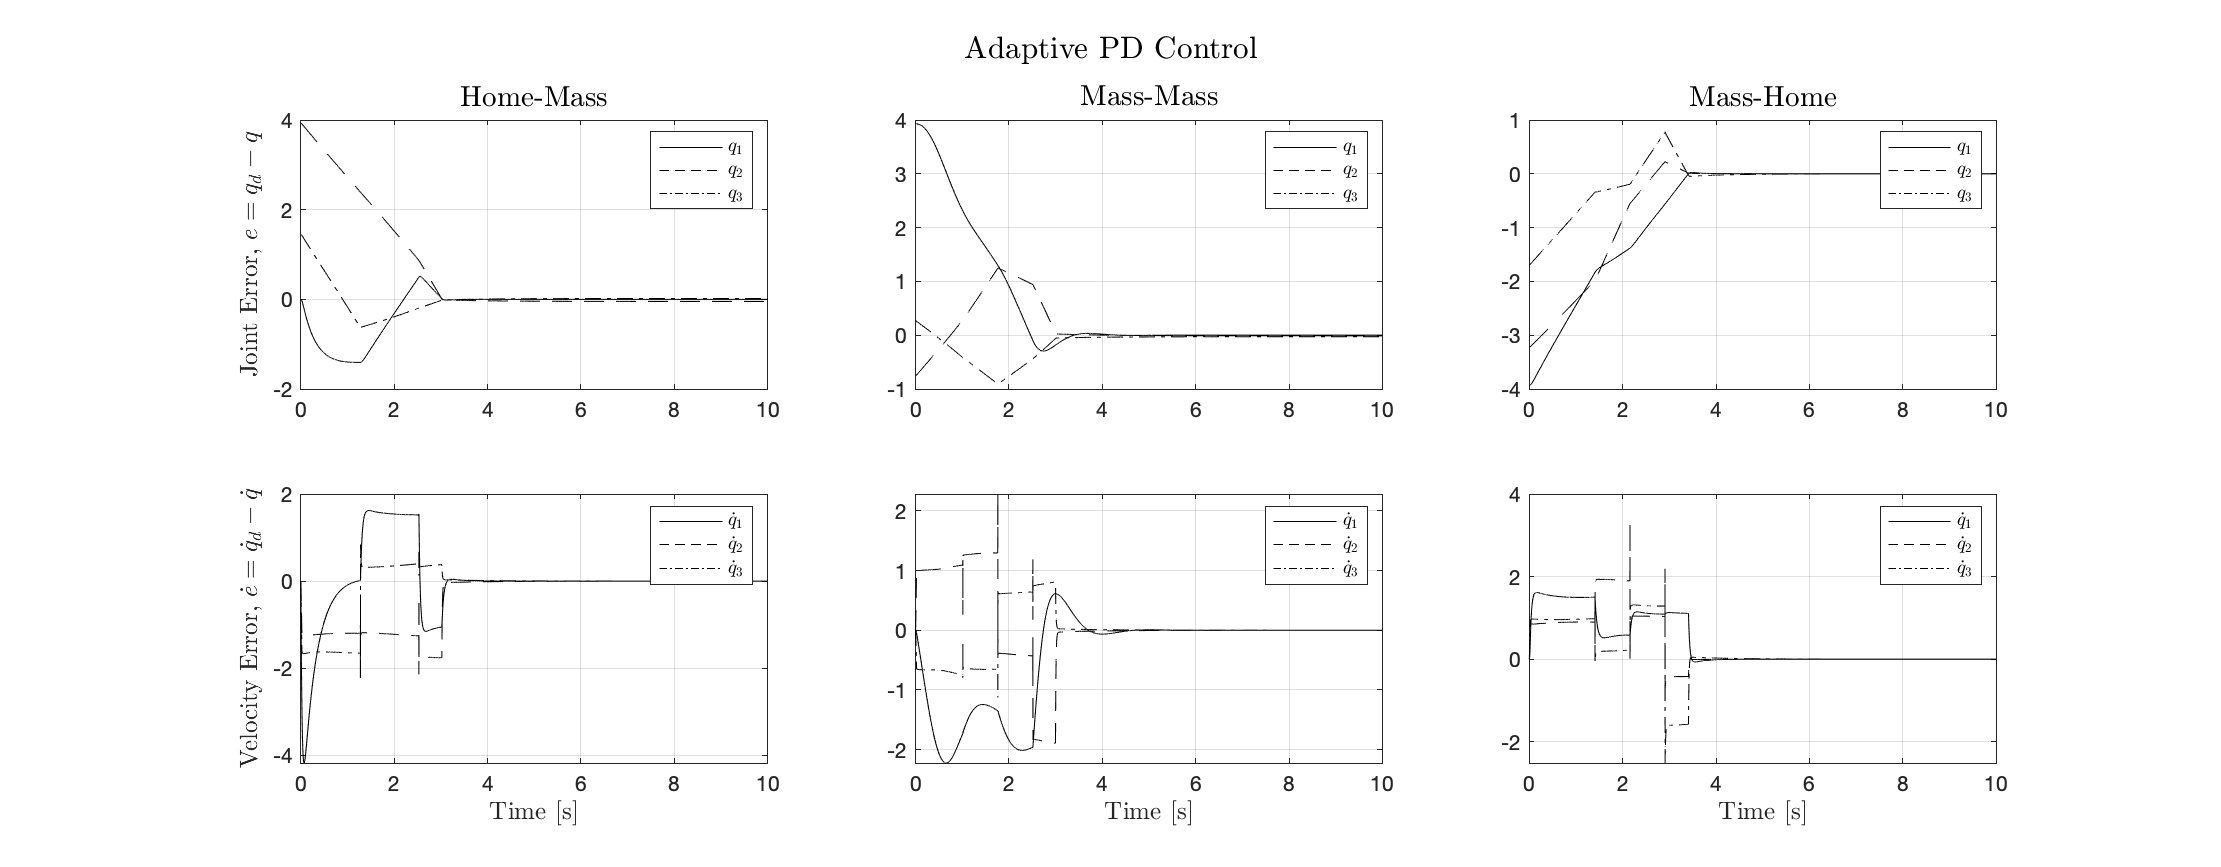
\includegraphics[width=\textwidth]{figures/mass10NNerrAPD.eps}
	\caption{Adaptive controller error in full simulation}
	\label{fig:nnerrapd}
\end{figure}
\begin{figure}[H]
	\centering
	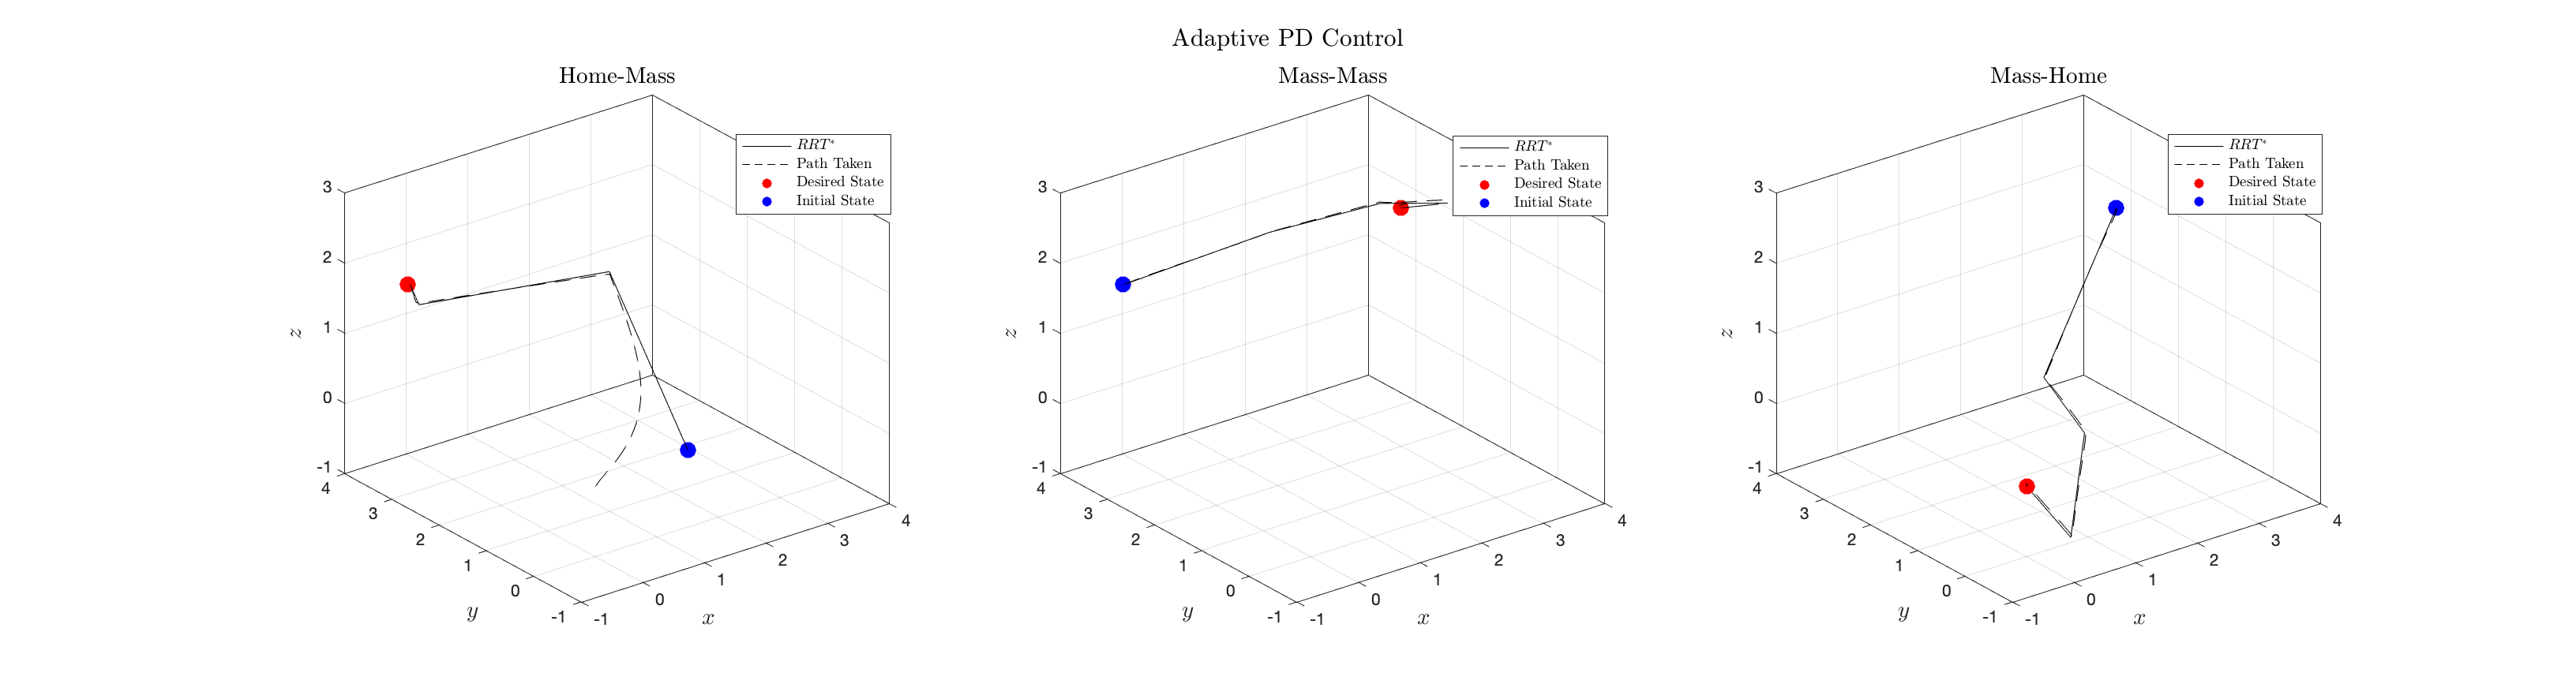
\includegraphics[width=\textwidth]{figures/mass10NNeetrajAPD.eps}
	\caption{End-effector trajectory with adaptive control}
	\label{fig:nntrajapd}
\end{figure}
\noindent We can see from Fig. \ref{fig:nntrajapd} that our initial error results in a false start position, however this error quickly decreases to zero as expected, and the trajectory is followed very tightly for the remainder of the simulation.

We then look at a mass estimated PD model, to observe the effects that an increase in mass has on the control.
\begin{figure}[H]
	\centering
	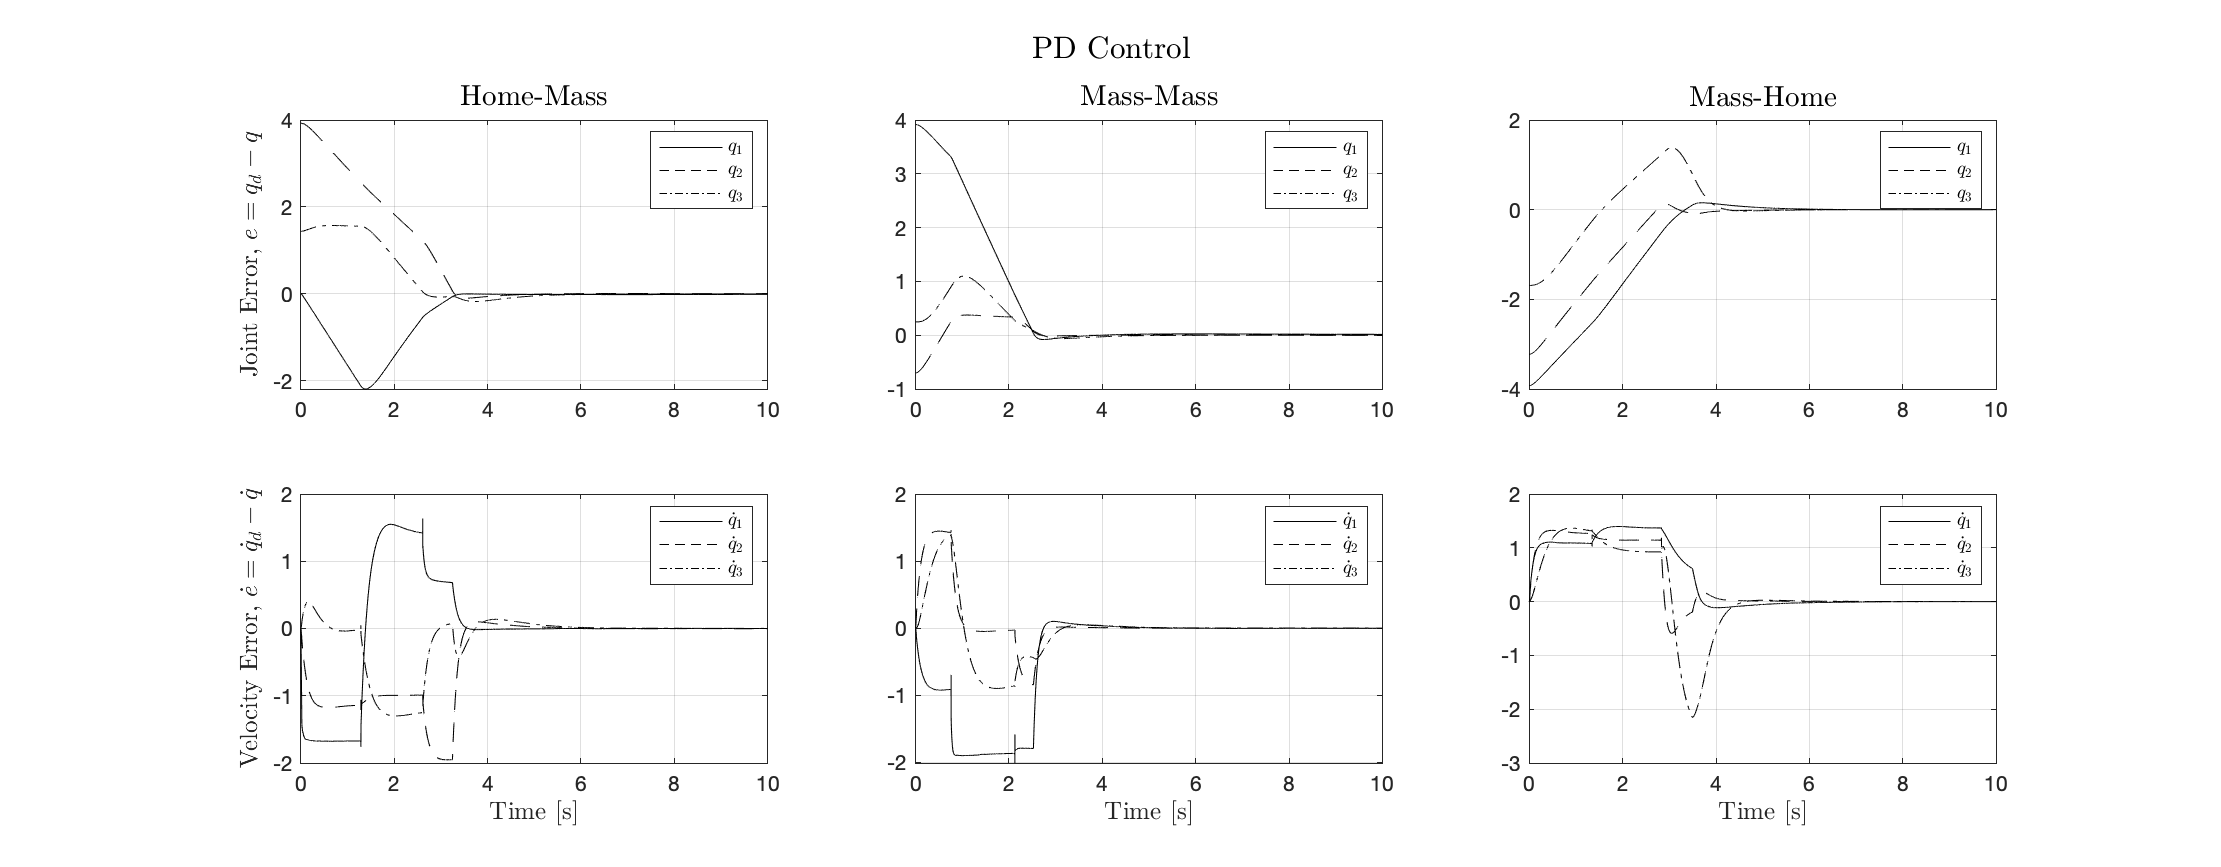
\includegraphics[width=\textwidth]{figures/mass10NNerrPD.eps}
	\caption{Mass estimated PD controller error in full simulation}
	\label{fig:nnerrpd}
\end{figure}
\begin{figure}[H]
	\centering
	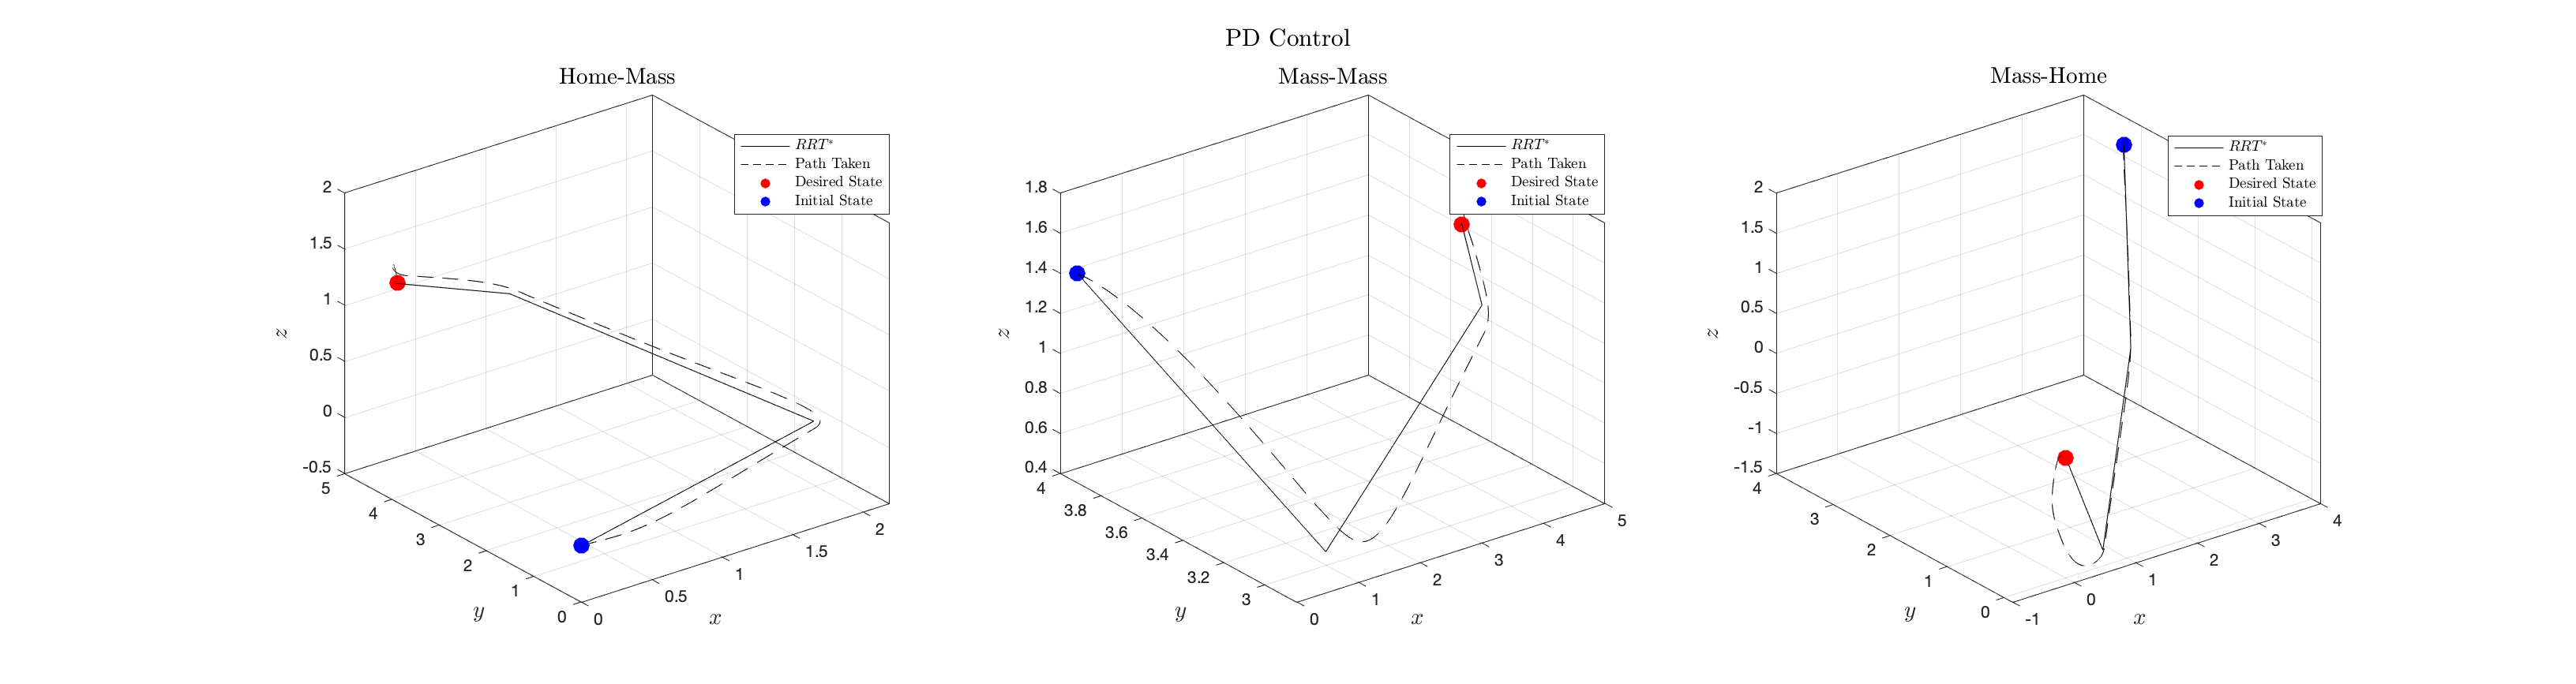
\includegraphics[width=\textwidth]{figures/mass10NNeetrajPD.eps}
	\caption{End-effector trajectory with mass estimated PD control}
	\label{fig:nntrajpd}
\end{figure}
\noindent In contrast to the adaptive model, the mass estimated PD controller places the end-effector in the desired start position.
However, we can easily see from Fig. \ref{fig:nntrajpd} that the PD control is not able to follow the desired trajectory as closely, and once the mass is picked up this issue worsens.

